\subsubsection{Feature Importance Metrics Comparison} \label{subsec:feature_importance_metrics_comparison}

For the evaluation the above mentioned feature importance methods were used.
In addition, for some of the methods in which a dataset was expected for calculation, both the train and the test datasets were used separately.
To evaluate the similarity of the feature importance values, the Spearman correlation coefficient was used.
Given the high number of experiments, the results for the LightGBM model are included in Fig.~\ref{fig:lgbm_correlation} for the linear dataset.
With standardization, the consistency of importance values can be enhanced across the different estimation methods,
as demonstrated in Subfig.~\ref{fig:lgbm_scaled_correlation}, while the correlation plot on Subfig.~\ref{fig:lgbm_nonscaled_correlation} for the model trained on non-standardized dataset emphasizes that without standardization tree specific importance values are less or not correlated with the other methods.
In both cases \emph{TREE\_SPLIT} importance is highlighted as the least correlated, the reason being that the model prefers splits on the continuous variables, as shown in Table~\ref{tab:lin_relative_importance}.
The main reason can be observed in Table~\ref{tab:lin_relative_importance}, where the relative importance values show that the model splits heavily on continuous variables, compared to the rest of features, even thogh the third and fourth lags have low average contribution by SHAP values and low PFI.

The PFI and SHAP values are more similar, only minor differences are present due to the usage of the test or train dataset in calculation.
Table \ref{tab:lin_relative_importance} illustrates the relative importance of the features for the linear dataset, allowing for a clearer comprehension.

% Correlation of results on LGBM
\begin{figure}[t]
    \centering
    \begin{subfigure}[t]{0.45\textwidth}
        \centering
        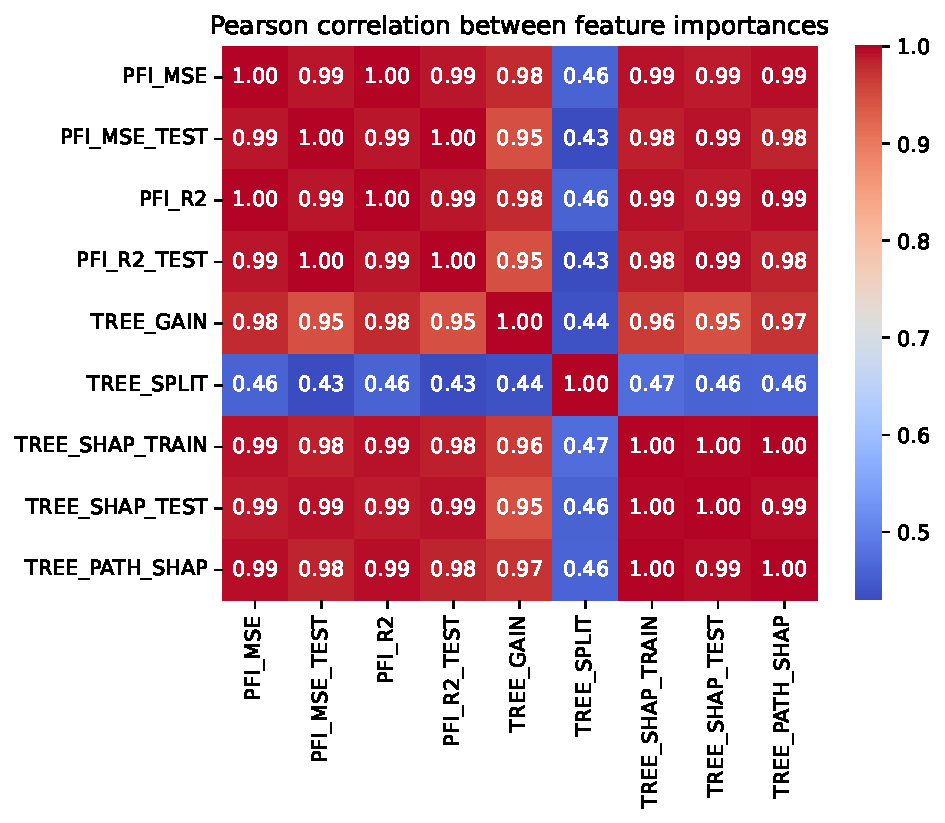
\includegraphics[width=\textwidth]{chapters/04_feature_importance_estimation/img/standardization/lin/lgbm_scaled/feature_importance_correlation}
        \caption{ With standardization}
        \label{fig:lgbm_scaled_correlation}
    \end{subfigure}
    \hfill
    \begin{subfigure}[t]{0.45\textwidth}
        \centering
        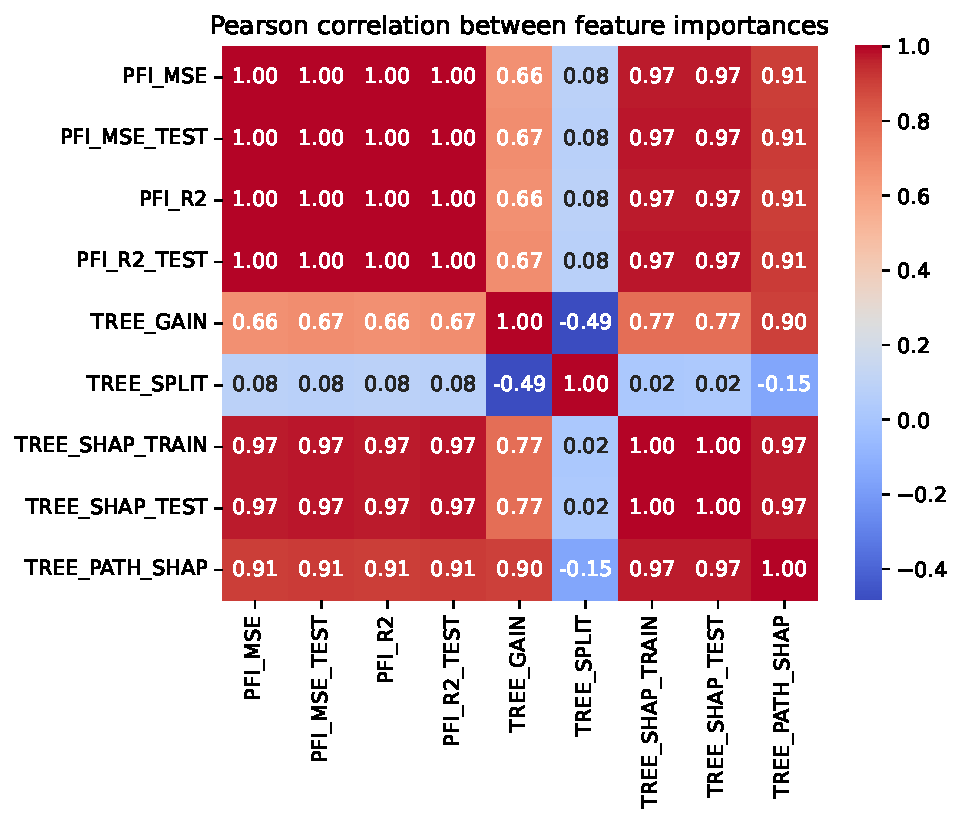
\includegraphics[width=\textwidth]{chapters/04_feature_importance_estimation/img/standardization/lin/lgbm_nonscaled/feature_importance_correlation}
        \caption{Without standardization}
        \label{fig:lgbm_nonscaled_correlation}
    \end{subfigure}
    \caption{Correlation of feature importance values for LightGBM model}
    \label{fig:lgbm_correlation}
\end{figure}






\begin{table}
    \centering
    \sisetup{table-auto-round}
    \caption{Relative importance of features for the LightGBM model with the linear dataset} \label{tab:lin_relative_importance}
    %round to 2 decimal places
    \begin{tabular}{|l|l|*{7}{S[table-format=2.2]|}}
        \toprule
        &                   & \rotatebox{65}{lag\_1}                                    & \rotatebox{65}{weather}                                   & \rotatebox{65}{lag\_2}                                    & \rotatebox{65}{lag\_4} & \rotatebox{65}{lag\_3} & \rotatebox{65}{holiday} & \rotatebox{65}{\_level} \\
        & Method            &                                                           &                                                           &                                                           &                                                           &                                                           &                                                          &                                                           \\
        \midrule
        \multirow[c]{9}{*}{\rotatebox{90}{Non-Standardized }}
        \rotatebox{90}{}
        & PFI\_MSE          & {\cellcolor[HTML]{B40426}} \color[HTML]{F1F1F1} 62.139293 & {\cellcolor[HTML]{6180E9}} \color[HTML]{F1F1F1} 7.787122 & {\cellcolor[HTML]{4961D2}} \color[HTML]{F1F1F1} 3.147222 & {\cellcolor[HTML]{3C4EC2}} \color[HTML]{F1F1F1} 0.430080 & {\cellcolor[HTML]{3C4EC2}} \color[HTML]{F1F1F1} 0.467753 & {\cellcolor[HTML]{3B4CC0}} \color[HTML]{F1F1F1} 0.174288 & {\cellcolor[HTML]{C5D6F2}} \color[HTML]{000000} 25.854242 \\
        & PFI\_MSE          & {\cellcolor[HTML]{B40426}} \color[HTML]{F1F1F1} 62.139293 & {\cellcolor[HTML]{6180E9}} \color[HTML]{F1F1F1} 7.787122 & {\cellcolor[HTML]{4961D2}} \color[HTML]{F1F1F1} 3.147222 & {\cellcolor[HTML]{3C4EC2}} \color[HTML]{F1F1F1} 0.430080 & {\cellcolor[HTML]{3C4EC2}} \color[HTML]{F1F1F1} 0.467753 & {\cellcolor[HTML]{3B4CC0}} \color[HTML]{F1F1F1} 0.174288 & {\cellcolor[HTML]{C5D6F2}} \color[HTML]{000000} 25.854242 \\
        \rotatebox{90}{}                           & PFI\_MSE\_TEST    & {\cellcolor[HTML]{B40426}} \color[HTML]{F1F1F1} 62.578422 & {\cellcolor[HTML]{6282EA}} \color[HTML]{F1F1F1} 8.005279 & {\cellcolor[HTML]{465ECF}} \color[HTML]{F1F1F1} 2.577019 & {\cellcolor[HTML]{3B4CC0}} \color[HTML]{F1F1F1} 0.100194 & {\cellcolor[HTML]{3B4CC0}} \color[HTML]{F1F1F1} 0.116158 & {\cellcolor[HTML]{3B4CC0}} \color[HTML]{F1F1F1} 0.107885 & {\cellcolor[HTML]{C7D7F0}} \color[HTML]{000000} 26.515042 \\
        \rotatebox{90}{}                           & PFI\_R2           & {\cellcolor[HTML]{B40426}} \color[HTML]{F1F1F1} 62.139293 & {\cellcolor[HTML]{6180E9}} \color[HTML]{F1F1F1} 7.787122 & {\cellcolor[HTML]{4961D2}} \color[HTML]{F1F1F1} 3.147222 & {\cellcolor[HTML]{3C4EC2}} \color[HTML]{F1F1F1} 0.430080 & {\cellcolor[HTML]{3C4EC2}} \color[HTML]{F1F1F1} 0.467753 & {\cellcolor[HTML]{3B4CC0}} \color[HTML]{F1F1F1} 0.174288 & {\cellcolor[HTML]{C5D6F2}} \color[HTML]{000000} 25.854242 \\
        \rotatebox{90}{}                           & PFI\_R2\_TEST     & {\cellcolor[HTML]{B40426}} \color[HTML]{F1F1F1} 62.578422 & {\cellcolor[HTML]{6282EA}} \color[HTML]{F1F1F1} 8.005279 & {\cellcolor[HTML]{465ECF}} \color[HTML]{F1F1F1} 2.577019 & {\cellcolor[HTML]{3B4CC0}} \color[HTML]{F1F1F1} 0.100194 & {\cellcolor[HTML]{3B4CC0}} \color[HTML]{F1F1F1} 0.116158 & {\cellcolor[HTML]{3B4CC0}} \color[HTML]{F1F1F1} 0.107885 & {\cellcolor[HTML]{C7D7F0}} \color[HTML]{000000} 26.515042 \\
        \rotatebox{90}{}                           & TREE\_GAIN        & {\cellcolor[HTML]{E1DAD6}} \color[HTML]{000000} 31.623648 & {\cellcolor[HTML]{4B64D5}} \color[HTML]{F1F1F1} 3.511285 & {\cellcolor[HTML]{4358CB}} \color[HTML]{F1F1F1} 1.785450 & {\cellcolor[HTML]{3B4CC0}} \color[HTML]{F1F1F1} 0.128045 & {\cellcolor[HTML]{4358CB}} \color[HTML]{F1F1F1} 1.871147 & {\cellcolor[HTML]{3B4CC0}} \color[HTML]{F1F1F1} 0.055824 & {\cellcolor[HTML]{B40426}} \color[HTML]{F1F1F1} 61.024600 \\
        \rotatebox{90}{}                           & TREE\_PATH\_SHAP  & {\cellcolor[HTML]{B40426}} \color[HTML]{F1F1F1} 38.511049 & {\cellcolor[HTML]{9FBFFF}} \color[HTML]{000000} 12.565807 & {\cellcolor[HTML]{688AEF}} \color[HTML]{F1F1F1} 6.781981 & {\cellcolor[HTML]{3B4CC0}} \color[HTML]{F1F1F1} 1.253256 & {\cellcolor[HTML]{4C66D6}} \color[HTML]{F1F1F1} 3.437702 & {\cellcolor[HTML]{3D50C3}} \color[HTML]{F1F1F1} 1.660050 & {\cellcolor[HTML]{CD423B}} \color[HTML]{F1F1F1} 35.790156 \\
        \rotatebox{90}{}                           & TREE\_SHAP\_TEST  & {\cellcolor[HTML]{B40426}} \color[HTML]{F1F1F1} 43.956162 & {\cellcolor[HTML]{98B9FF}} \color[HTML]{000000} 13.523832 & {\cellcolor[HTML]{7295F4}} \color[HTML]{F1F1F1} 8.938335 & {\cellcolor[HTML]{3B4CC0}} \color[HTML]{F1F1F1} 1.497947 & {\cellcolor[HTML]{3E51C5}} \color[HTML]{F1F1F1} 2.077869 & {\cellcolor[HTML]{3C4EC2}} \color[HTML]{F1F1F1} 1.711196 & {\cellcolor[HTML]{F5C2AA}} \color[HTML]{000000} 28.294658 \\
        \rotatebox{90}{}                           & TREE\_SHAP\_TRAIN & {\cellcolor[HTML]{B40426}} \color[HTML]{F1F1F1} 43.886278 & {\cellcolor[HTML]{96B7FF}} \color[HTML]{000000} 13.166581 & {\cellcolor[HTML]{7597F6}} \color[HTML]{F1F1F1} 9.204476 & {\cellcolor[HTML]{3B4CC0}} \color[HTML]{F1F1F1} 1.663227 & {\cellcolor[HTML]{3E51C5}} \color[HTML]{F1F1F1} 2.113341 & {\cellcolor[HTML]{3B4CC0}} \color[HTML]{F1F1F1} 1.577080 & {\cellcolor[HTML]{F5C1A9}} \color[HTML]{000000} 28.389017 \\
        \rotatebox{90}{}                           & TREE\_SPLIT       & {\cellcolor[HTML]{CA3B37}} \color[HTML]{F1F1F1} 20.514056 & {\cellcolor[HTML]{B40426}} \color[HTML]{F1F1F1} 21.767068 & {\cellcolor[HTML]{E26952}} \color[HTML]{F1F1F1} 18.746988 & {\cellcolor[HTML]{ED8366}} \color[HTML]{F1F1F1} 17.574297 & {\cellcolor[HTML]{E67259}} \color[HTML]{F1F1F1} 18.329317 & {\cellcolor[HTML]{5A78E4}} \color[HTML]{F1F1F1} 2.618474 & {\cellcolor[HTML]{3B4CC0}} \color[HTML]{F1F1F1} 0.449799 \\
        \cline{1-10}
        \multirow[c]{9}{*}{\rotatebox{90}{Standardized}} & PFI\_MSE          & {\cellcolor[HTML]{B40426}} \color[HTML]{F1F1F1} 47.037873 & {\cellcolor[HTML]{D95847}} \color[HTML]{F1F1F1} 41.859593 & {\cellcolor[HTML]{6384EB}} \color[HTML]{F1F1F1} 6.601536 & {\cellcolor[HTML]{4257C9}} \color[HTML]{F1F1F1} 1.631846 & {\cellcolor[HTML]{4257C9}} \color[HTML]{F1F1F1} 1.610705 & {\cellcolor[HTML]{3C4EC2}} \color[HTML]{F1F1F1} 0.739083 & {\cellcolor[HTML]{3B4CC0}} \color[HTML]{F1F1F1} 0.519364 \\
        \rotatebox{90}{}                           & PFI\_MSE\_TEST    & {\cellcolor[HTML]{D44E41}} \color[HTML]{F1F1F1} 45.292131 & {\cellcolor[HTML]{B40426}} \color[HTML]{F1F1F1} 49.903083 & {\cellcolor[HTML]{5470DE}} \color[HTML]{F1F1F1} 4.216054 & {\cellcolor[HTML]{3B4CC0}} \color[HTML]{F1F1F1} -0.007306 & {\cellcolor[HTML]{3B4CC0}} \color[HTML]{F1F1F1} 0.000794 & {\cellcolor[HTML]{3E51C5}} \color[HTML]{F1F1F1} 0.582664 & {\cellcolor[HTML]{3B4CC0}} \color[HTML]{F1F1F1} 0.012579 \\
        \rotatebox{90}{}                           & PFI\_R2           & {\cellcolor[HTML]{B40426}} \color[HTML]{F1F1F1} 47.037873 & {\cellcolor[HTML]{D95847}} \color[HTML]{F1F1F1} 41.859593 & {\cellcolor[HTML]{6384EB}} \color[HTML]{F1F1F1} 6.601536 & {\cellcolor[HTML]{4257C9}} \color[HTML]{F1F1F1} 1.631846 & {\cellcolor[HTML]{4257C9}} \color[HTML]{F1F1F1} 1.610705 & {\cellcolor[HTML]{3C4EC2}} \color[HTML]{F1F1F1} 0.739083 & {\cellcolor[HTML]{3B4CC0}} \color[HTML]{F1F1F1} 0.519364 \\
        \rotatebox{90}{}                           & PFI\_R2\_TEST     & {\cellcolor[HTML]{D44E41}} \color[HTML]{F1F1F1} 45.292131 & {\cellcolor[HTML]{B40426}} \color[HTML]{F1F1F1} 49.903083 & {\cellcolor[HTML]{5470DE}} \color[HTML]{F1F1F1} 4.216054 & {\cellcolor[HTML]{3B4CC0}} \color[HTML]{F1F1F1} -0.007306 & {\cellcolor[HTML]{3B4CC0}} \color[HTML]{F1F1F1} 0.000794 & {\cellcolor[HTML]{3E51C5}} \color[HTML]{F1F1F1} 0.582664 & {\cellcolor[HTML]{3B4CC0}} \color[HTML]{F1F1F1} 0.012579 \\
        \rotatebox{90}{}                           & TREE\_GAIN        & {\cellcolor[HTML]{B40426}} \color[HTML]{F1F1F1} 55.761504 & {\cellcolor[HTML]{F5C4AC}} \color[HTML]{000000} 35.050195 & {\cellcolor[HTML]{5B7AE5}} \color[HTML]{F1F1F1} 6.157949 & {\cellcolor[HTML]{3F53C6}} \color[HTML]{F1F1F1} 1.193052 & {\cellcolor[HTML]{3F53C6}} \color[HTML]{F1F1F1} 1.146824 & {\cellcolor[HTML]{3C4EC2}} \color[HTML]{F1F1F1} 0.488410 & {\cellcolor[HTML]{3B4CC0}} \color[HTML]{F1F1F1} 0.202067 \\
        \rotatebox{90}{}                           & TREE\_PATH\_SHAP  & {\cellcolor[HTML]{B40426}} \color[HTML]{F1F1F1} 40.319856 & {\cellcolor[HTML]{D44E41}} \color[HTML]{F1F1F1} 36.685986 & {\cellcolor[HTML]{8FB1FE}} \color[HTML]{000000} 11.498906 & {\cellcolor[HTML]{4257C9}} \color[HTML]{F1F1F1} 2.505798 & {\cellcolor[HTML]{445ACC}} \color[HTML]{F1F1F1} 2.876513 & {\cellcolor[HTML]{536EDD}} \color[HTML]{F1F1F1} 4.581488 & {\cellcolor[HTML]{3B4CC0}} \color[HTML]{F1F1F1} 1.531454 \\
        \rotatebox{90}{}                           & TREE\_SHAP\_TEST  & {\cellcolor[HTML]{CB3E38}} \color[HTML]{F1F1F1} 37.328384 & {\cellcolor[HTML]{B40426}} \color[HTML]{F1F1F1} 39.715190 & {\cellcolor[HTML]{90B2FE}} \color[HTML]{000000} 11.569779 & {\cellcolor[HTML]{3F53C6}} \color[HTML]{F1F1F1} 2.426402 & {\cellcolor[HTML]{4257C9}} \color[HTML]{F1F1F1} 2.651869 & {\cellcolor[HTML]{516DDB}} \color[HTML]{F1F1F1} 4.604555 & {\cellcolor[HTML]{3B4CC0}} \color[HTML]{F1F1F1} 1.703821 \\
        \rotatebox{90}{}                           & TREE\_SHAP\_TRAIN & {\cellcolor[HTML]{B40426}} \color[HTML]{F1F1F1} 39.103839 & {\cellcolor[HTML]{C83836}} \color[HTML]{F1F1F1} 36.997465 & {\cellcolor[HTML]{98B9FF}} \color[HTML]{000000} 12.234161 & {\cellcolor[HTML]{4358CB}} \color[HTML]{F1F1F1} 2.742010 & {\cellcolor[HTML]{455CCE}} \color[HTML]{F1F1F1} 2.900807 & {\cellcolor[HTML]{516DDB}} \color[HTML]{F1F1F1} 4.448172 & {\cellcolor[HTML]{3B4CC0}} \color[HTML]{F1F1F1} 1.573546 \\
        \rotatebox{90}{}                           & TREE\_SPLIT       & {\cellcolor[HTML]{C43032}} \color[HTML]{F1F1F1} 18.930277 & {\cellcolor[HTML]{BE242E}} \color[HTML]{F1F1F1} 19.216810 & {\cellcolor[HTML]{C73635}} \color[HTML]{F1F1F1} 18.825215 & {\cellcolor[HTML]{B40426}} \color[HTML]{F1F1F1} 19.723018 & {\cellcolor[HTML]{D65244}} \color[HTML]{F1F1F1} 18.013372 & {\cellcolor[HTML]{3B4CC0}} \color[HTML]{F1F1F1} 2.521490 & {\cellcolor[HTML]{3E51C5}} \color[HTML]{F1F1F1} 2.769819 \\

        \cline{1-10}
        \bottomrule
    \end{tabular}
\end{table}


%\color{red}
%Todo: compare the feature importance metrics:
%%- Include correlation plot for the feature importances
%- Discuss and include the violin plots as means to show the distribution of the importance values
%- Tree path perturbationn SHAP - value difference to interventional - Create table with limited results
%%- include all results in appendix just for discussion
%\color{black}

\subsubsection{Feature scaling effect on importance measures} \label{subsec:feature_scaling_effect}
Feature scaling affects the models this way, the importance values are shifted to other features as show in~\ref{tab:lin_relative_importance}.
Without standardization, the models rely heavily on the `\_level` feature, which is the identifier of the time series,
but the `TREE_SPLIT` values are low signaling that only a few splits are made to differentiate the series causing low generalization.

The violin plots of SHAP values for a single series, shown in Figure~\ref{fig:sc_nsc_lgbm_s1} for the LightGBM model and Figure~\ref{fig:sc_nsc_rf_s1} for the Random Forest model, illustrate how feature importance values differ between standardized and non-standardized datasets.
Without scaling the `_level` values have much larger magnitude, even dominating as in case of the Random Forest model for the series 3 in Figure~\ref{fig:fig:sc_nsc_rf_lgbm_s3}.
With the standardized input features, the importance values are more evenly distributed, with weather and holiday effect having a higher importance above the `lag_3` and `lag_4` which should have low direct impact on the target.
However, the scaling also has a disadvantage that the importance values are not as intuitive,
as the values are not on the same scale as the original sales volumes.
SHAP values representing the change in prediction value in the original feature space, can be important for a decision maker, as they could provide the potential growth or decrease in sales volume.

\begin{figure}
    \centering
    \begin{subfigure}[t]{0.45\textwidth}
        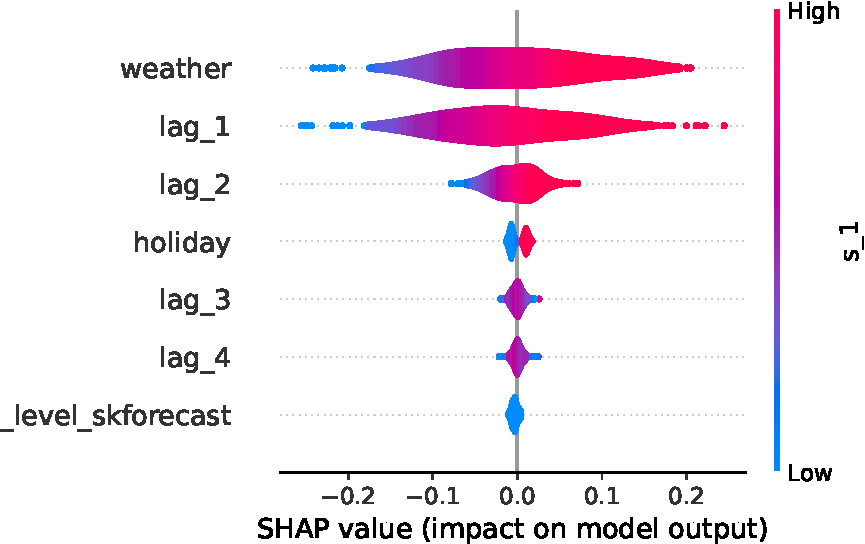
\includegraphics[width=\textwidth]{chapters/04_feature_importance_estimation/img/standardization/lin/lgbm_scaled/shap_violin_s_1}
        \caption{Standardized}
    \end{subfigure}
    \hfill
    \begin{subfigure}[t]{0.45\textwidth}
        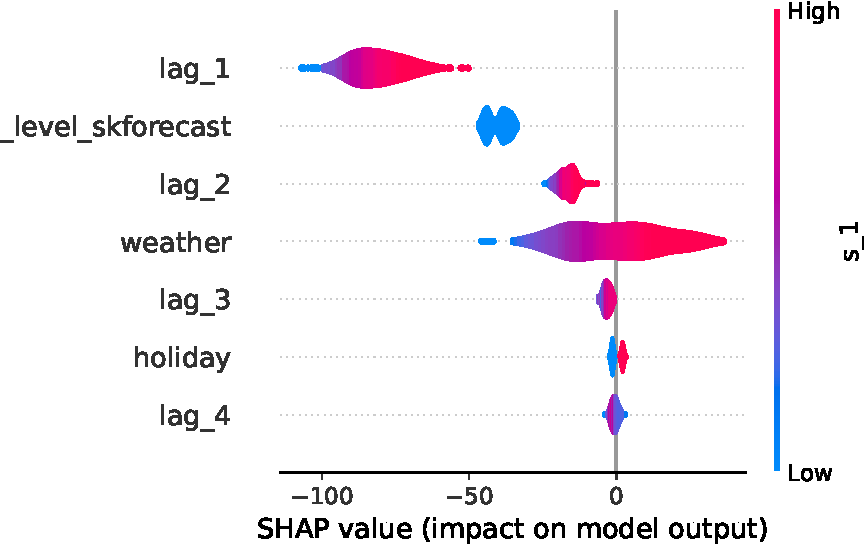
\includegraphics[width=\textwidth]{chapters/04_feature_importance_estimation/img/standardization/lin/lgbm_nonscaled/shap_violin_s_1}
        \caption{Non-standardized}
    \end{subfigure}
    \caption{Feature importance values for LightGBM model for series 1}\label{fig:sc_nsc_lgbm_s1}
\end{figure}

\begin{figure}
    \centering
    \begin{subfigure}[b]{0.45\textwidth}
        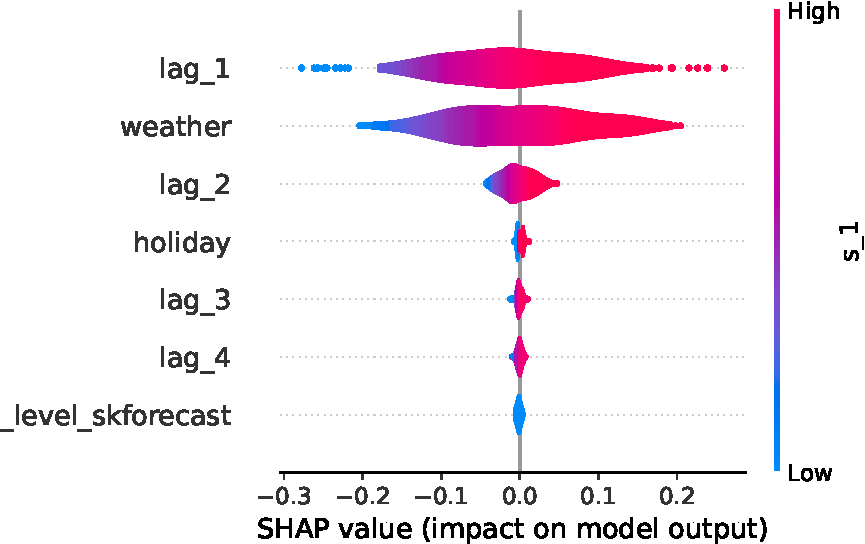
\includegraphics[width=\textwidth]{chapters/04_feature_importance_estimation/img/standardization/lin/rf_forecaster_scaled/shap_violin_s_1}
        \caption{Standardized}
    \end{subfigure}
    \hfill
    \begin{subfigure}[b]{0.45\textwidth}
        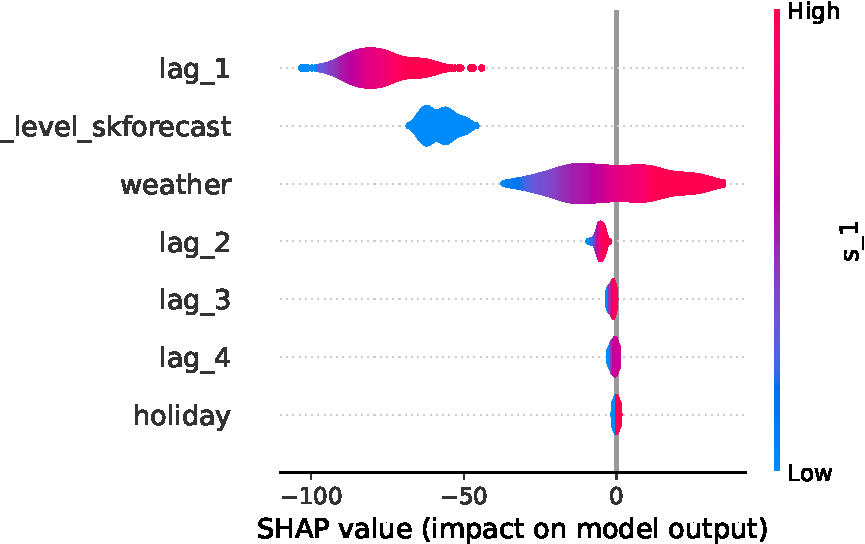
\includegraphics[width=\textwidth]{chapters/04_feature_importance_estimation/img/standardization/lin/rf_forecaster_nonscaled/shap_violin_s_1}
        \caption{Non-standardized}
    \end{subfigure}
    \caption{Feature importance values for Random Forest model for series 1}\label{fig:sc_nsc_rf_s1}
\end{figure}

\begin{figure}
    \centering
    \begin{subfigure}[b]{0.45\textwidth}
        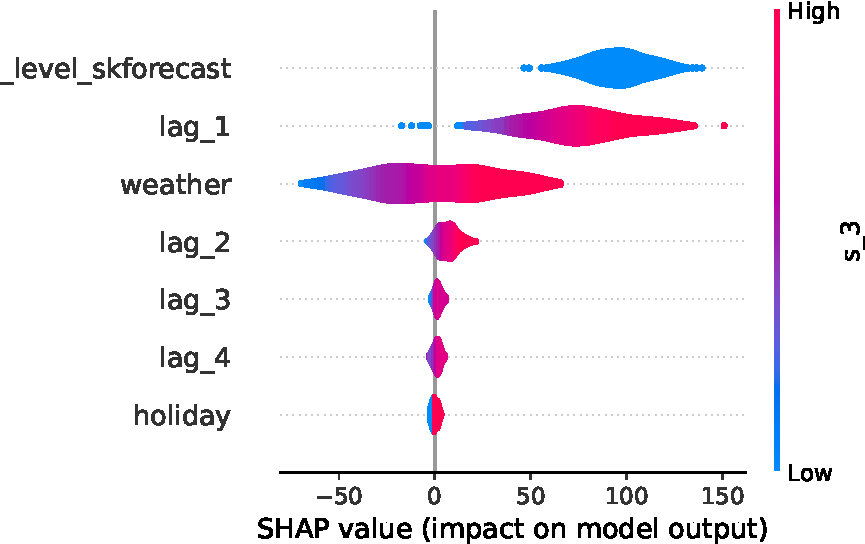
\includegraphics[width=\textwidth]{chapters/04_feature_importance_estimation/img/standardization/lin/rf_forecaster_nonscaled/shap_violin_s_3}
        \caption{Random forest}
    \end{subfigure}
    \hfill
    \begin{subfigure}[b]{0.45\textwidth}
        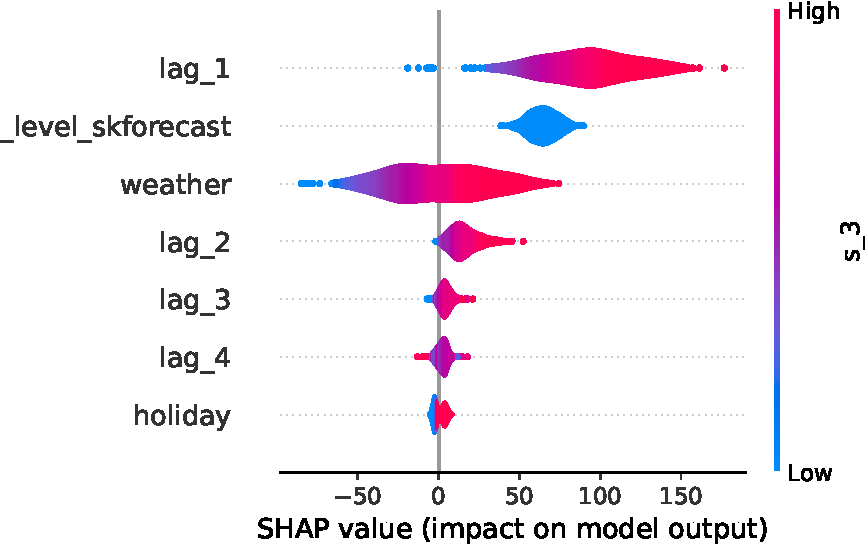
\includegraphics[width=\textwidth]{chapters/04_feature_importance_estimation/img/standardization/lin/lgbm_nonscaled/shap_violin_s_3}
        \caption{LightGBM}
    \end{subfigure}
    \caption{Feature importance values for Random Forest and LightGBM models without standardization for series 3}\label{fig:fig:sc_nsc_rf_lgbm_s3}
\end{figure}

\subsubsection{Correlation of features and extrapolation} \label{subsec:correlation_of_features_and_importance}

\begin{figure}[t]
    \centering
    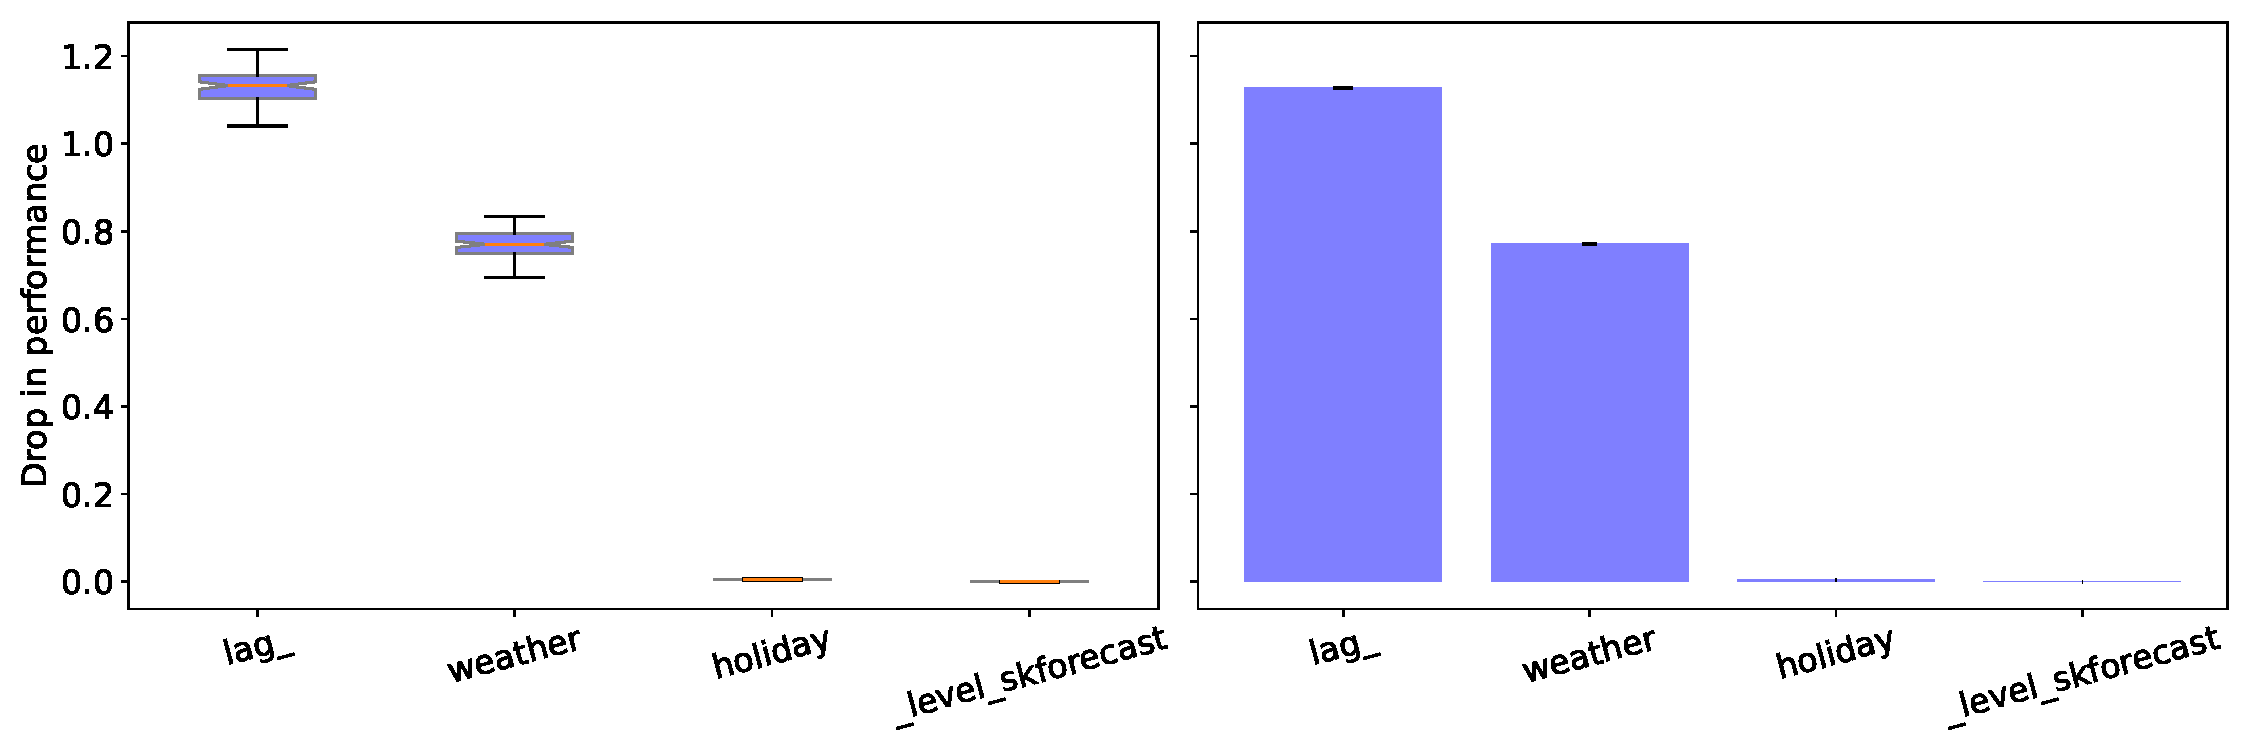
\includegraphics[width=\textwidth]{chapters/04_feature_importance_estimation/img/standardization/lin/rf_forecaster_scaled_grouped_permutation_importance}
    \caption{Grouped permutation feature importance Random Forest model with standardization}
    \label{fig:rf_grouped_permutation_importance}
\end{figure}

\begin{table}
    \centering
    \caption{Relative feature importance for grouped PFI for the linear combined dataset.} \label{tab:lin_grouped_relative}
    \begin{tabular}{lrrrr}
        \toprule
        & lgbm\_scaled & lgbm\_nonscaled & rf\_scaled & rf\_nonscaled \\
        \midrule
        \_level\_skforecast & 0.000103     & 0.196046        & -0.000194              & 0.439479                  \\
        holiday             & 0.004765     & 0.000798        & 0.002362               & 0.000293                  \\
        lag\_               & 0.587014     & 0.743967        & 0.592377               & 0.501273                  \\
        weather             & 0.408118     & 0.059189        & 0.405455               & 0.058956                  \\
        \bottomrule
    \end{tabular}
\end{table}


\begin{table}
    \centering
    \caption{Relative feature importance for grouped PFI for the non-linear combined dataset.} \label{tab:nonlin_grouped_relative}
    \begin{tabular}{lrrrr}
        \toprule
        & lgbm\_scaled & lgbm\_nonscaled & rf\_scaled & rf\_nonscaled \\
        \midrule
        \_level\_skforecast    & 0.018005     & 0.029358        & 0.011419   & 0.010066      \\
        day\_of\_year          & 0.198566     & 0.021532        & 0.070868   & 0.006378      \\
        holiday\_trend\_factor & 0.029211     & 0.004774        & 0.016281   & 0.002154      \\
        lag\_                  & 0.381743     & 0.868834        & 0.571649   & 0.918375      \\
        weekend\_trend\_factor & 0.372476     & 0.075502        & 0.329783   & 0.063028      \\
        \bottomrule
    \end{tabular}
\end{table}



In Fig.~\ref{fig:rf_grouped_permutation_importance} the grouped PFI by the coefficient of determination for the Random Forest model with standardisation is shown.
As expected, the importance of the grouped lag variables is the highest,followed by the exogenous variables.
The relative importances are shown in Table~\ref{tab:lin_grouped_relative} for linear and Table~\ref{tab:nonlin_grouped_relative} for non-linear datasets.
In the case of the linear dataset by scaling, the importance of the lag values are reduced, but the relative importance for the two models is similar.
The value of approximately 0.6 for the lag variable makes sense, as the `lag\_1` contributed 0.6 to the target in data generation
and the `lag\_2` variable has its contribution reduced by the `lag\_1` variable.

The results of the non-linear dataset in Table~\ref{tab:nonlin_grouped_relative}, the importance of lag variables is the highest showing that the model relies almost solely on the lagged values to make predictions, highlighting the fact of the importance of data scaling.